\documentclass{article}
\usepackage[top=2cm,bottom=2cm,left=2cm,right=2cm]{geometry}
\usepackage{amsmath, amsthm}
\usepackage{tikz}
\usepackage{hyperref}

\usepackage{datetime}
\newdateformat{petsa}{\the\day\ \shortmonthname[\the\month] \the\year}

\theoremstyle{plain}
\newtheorem{definition}{Definition}[section]
\newtheorem{theorem}{Theorem}[section]
\newtheorem{lemma}[theorem]{Lemma}
\newtheorem{conjecture}[theorem]{Conjecture}

\theoremstyle{remark}
\newtheorem*{remark}{Remark}

\title{Description and Proof of Correctness of \texttt{treedrawing}}
\author{poypoyan}
\date{\petsa\today}

\begin{document}

\maketitle

\begin{abstract}
This note contains an overview of my Github repo \texttt{treedrawing} \cite{treedrawing}, which is a naive algorithm that neatly draws rooted trees. Then a proof of correctness of the algorithm is presented.
\end{abstract}

\section{Definitions}
We start by introducing some standard and non-standard terminologies:
\begin{definition}
A \textbf{rooted tree} is a triple $T=(V, E, r)$ where $(V, E)$ is a tree (a graph without cycles), and $r \in V$ is called the \textbf{root}.
\end{definition}
\begin{remark}
We adopt terminologies from computer science: we call $V$ the set of \textbf{nodes} (instead of vertices), and $E$ the set of \textbf{branches} (instead of edges).
\end{remark}
\begin{definition}
For nodes $x, y \in V$ connected by a branch, $x$ is the \textbf{parent} of $y$ and $y$ is a \textbf{child} of $x$ if $x$ has closer path to the root than $y$. 
\end{definition}
\begin{definition}
A \textbf{leaf} is a node that does not have a child.
\end{definition}
\begin{definition}
A non-root node is \textbf{minor} iff it is the only child of its parent and it has exactly one child node. A node is \textbf{major} iff it is the root or it is not minor. 
\end{definition}
\begin{definition}
The \textbf{sub-rooted tree} by a major node $x \in V$ is a rooted tree $T'=(V', E', x)$ consisting of $x$ itself (as root) and all of its the `descendant' nodes.
\end{definition}
\begin{remark}
(1) The sub-rooted tree by the root node is the whole rooted tree. (2) The sub-rooted tree by the leaf node is the trivial branch-less tree with itself as the only node.
\end{remark}
\begin{definition}\label{weight}
The \textbf{weight} of a major node is the number of major nodes of the sub-rooted tree by that node. The weight of a minor node is 0.
\end{definition}
\begin{remark}
The weight of every leaf node is 1.
\end{remark}

We show the converse of the last sentence in Definition \ref{weight}: all nodes of weight 0 are minor. This is equivalent to the statement that all major nodes have weights of at least 1. This is indeed the case because the major node itself is contained in the sub-rooted tree by itself. In conclusion, a node is minor iff its weight is 0.

To aid in understanding the concepts, an example rooted tree is provided in Figure \ref{rooted-tree}.

\begin{figure}[htbp]
	\centering
	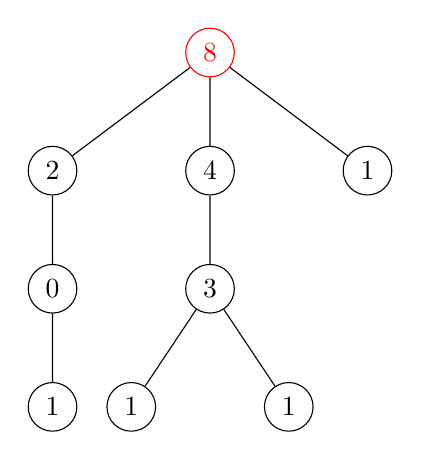
\begin{tikzpicture}[nodes = {draw, circle}]
		\node [red] {8} [sibling distance = 2cm]
		child {node {2}
			child {node {0}
				child {node {1}}
			}
		}
		child {node {4}
			child {node {3}
				child {node {1}}
				child {node {1}}
			}
		}
		child {node {1}};
	\end{tikzpicture}
	\caption{Example rooted tree with red-colored node as the root. The number in node indicate its weight.}
	\label{rooted-tree}
\end{figure}

\section{Algorithm Description}
The algorithm consists of three main functions that are executed in order: (1) \texttt{analyzeNode}, which records relevant information for each node recursively, (2) \texttt{setInitCoord}, which sets initial coordinates to each node recursively, and (3) \texttt{fixCoord}, which fixes coordinates of nodes so that there are no nodes with same location.

\subsection{Function \texttt{analyzeNode}}
The main input of the algorithm is any data with a structure of rooted tree. Note that nodes in the input data must be \textit{labelled}. What the \texttt{analyzeNode} function mainly does is to perform tree traversal on the data and record the following information:

\begin{itemize}
	\item \texttt{connecNodes} is an array of arrays of natural numbers. An index \texttt{idx} in \texttt{connecNodes[idx]} corresponds to a node (with \texttt{idx = 0} being the root). Now \texttt{connecNodes[idx]} itself is the array of indices that correspond to the \textit{children} of the \texttt{idx} node. If the \texttt{idx} node is a leaf, then \texttt{connecNodes[idx]} is the empty array.
	\item \texttt{labelDict} is a function that aligns node \textit{labels} (strings) to indices for \texttt{connecNodes}, \texttt{weightNodes}, and \texttt{majorNodes}.
	\item \texttt{weightNodes} is an array of natural numbers. Like in \texttt{connecNodes}, an index \texttt{idx} in \texttt{weightNodes[idx]} corresponds to a node (with \texttt{idx = 0} being the root). Now \texttt{weightNodes[idx]} itself is the weight of the \texttt{idx} node.
	\item \texttt{majorNodes} is an array of objects. Like in \texttt{connecNodes}, an index \texttt{idx} in \texttt{majorNodes[idx]} corresponds to a node (with \texttt{idx = 0} being the root). Now for major nodes, \texttt{majorNodes[idx]} itself is the array of major nodes along the (unique) path from the root to the \texttt{idx} node (\texttt{idx} itself excluded). Since the root has no parent, \texttt{majorNodes[0]} is always the empty array. For minor nodes, \texttt{majorNodes[idx]} is the \textit{null} object.
\end{itemize}

\subsection{Function \texttt{setInitCoord}}
[To be continued.]
\subsection{Function \texttt{fixCoord}}
[To be continued.]
\section{Proof of Correctness}
[To be continued.]

\bibliographystyle{plain}
\bibliography{treedrawing}
\end{document}